\begin{itemize}
    \item A decision tree classifier is a recursive partition-based tree model that predicts the class $y_i$ for each point $x_i$.
    \item A decision tree uses axis-parallel hyperplanes.
    \item To classify a new test point we have to recursively evaluate which half-space it belongs to until we reach a leaf node in the decision tree, at which point we predict its class as the label of the leaf.
    \item Advantages include easily interpretable models, supports multi-class and handles both numeric and categoric data. Disadvantages is it can cause over fitting if used bad threshold values for input.
\begin{figure}[H]
\centerline{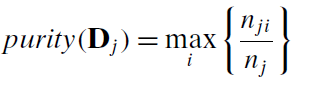
\includegraphics[width=0.4\textwidth]{Figures/dt1}}
\caption{\label{fig:figure}Purity Rule}
\end{figure}
\subsubsection{Split Point Measures: Information Gain}
\begin{figure}[H]
    \centering
    \begin{minipage}{0.6\textwidth}
        \centering
        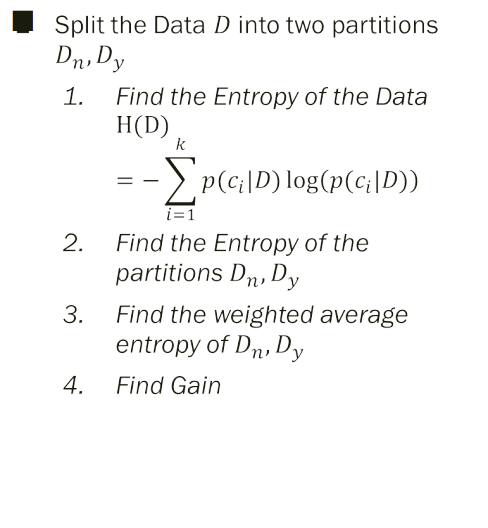
\includegraphics[width=0.9\textwidth]{Figures/dt2.png} % first figure itself
        \caption{Procedure}
    \end{minipage}\hfill
    \begin{minipage}{0.4\textwidth}
        \centering
        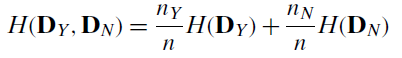
\includegraphics[width=\textwidth]{Figures/dt3.png} % second figure itself
        \caption{Split Entropy}
    \end{minipage}
        \begin{minipage}{0.4\textwidth}
        \centering
        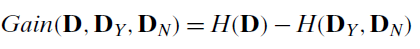
\includegraphics[width=\textwidth]{Figures/dt4.png} % second figure itself
        \caption{Gain}
    \end{minipage}
\end{figure}
\textbf{The Higher the better}
\subsubsection{Split Point Measures: Gini-Index}
\begin{figure}[H]
    \centering
    \begin{minipage}{0.5\textwidth}
        \centering
        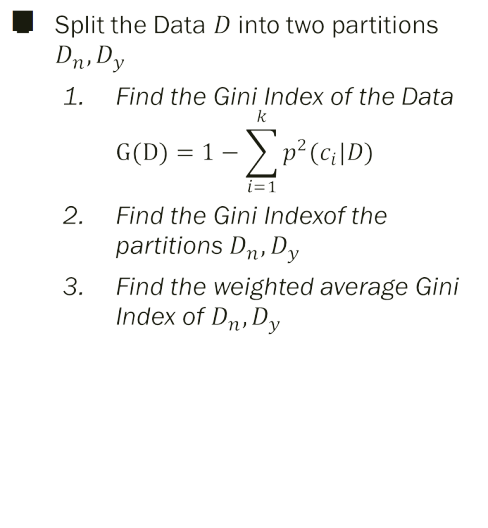
\includegraphics[width=\textwidth]{Figures/dt5.png} % first figure itself
        \caption{Procedure}
    \end{minipage}\hfill
    \begin{minipage}{0.5\textwidth}
        \centering
        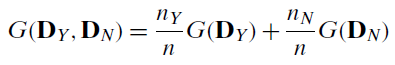
\includegraphics[width=\textwidth]{Figures/dt6.png} % second figure itself
        \caption{Weighted Gini-Index for Split Point}
    \end{minipage}
\end{figure}
\textbf{The Lower the better}
\textbf{The Gini coefficient provides an index to measure impurity}
\begin{figure}[H]
\centerline{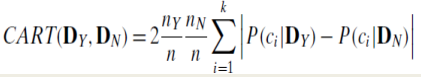
\includegraphics[width=0.7\textwidth]{Figures/cart}}
\caption{\label{fig:figure}Cart Measure Rule}
\end{figure}

    \item For a numeric attribute x, How to find the split value?Use midpoint of the possible distinct values for x because it is bounded by the number of distinct points which is at most all points. 
\end{itemize}

\subsubsection{Numeric Example}
\begin{figure}[H]
\centerline{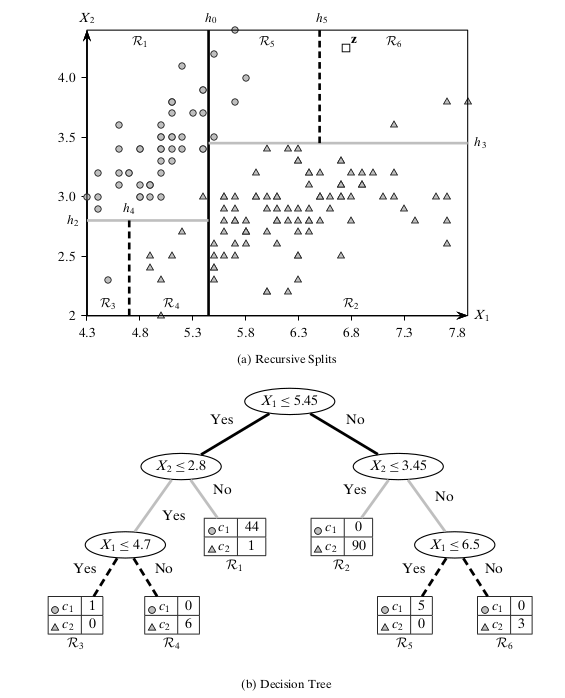
\includegraphics[width=\textwidth]{Figures/dt8}}
\caption{\label{fig:figure}Data and Generated Tree}
\end{figure}
\begin{figure}[H]
\centerline{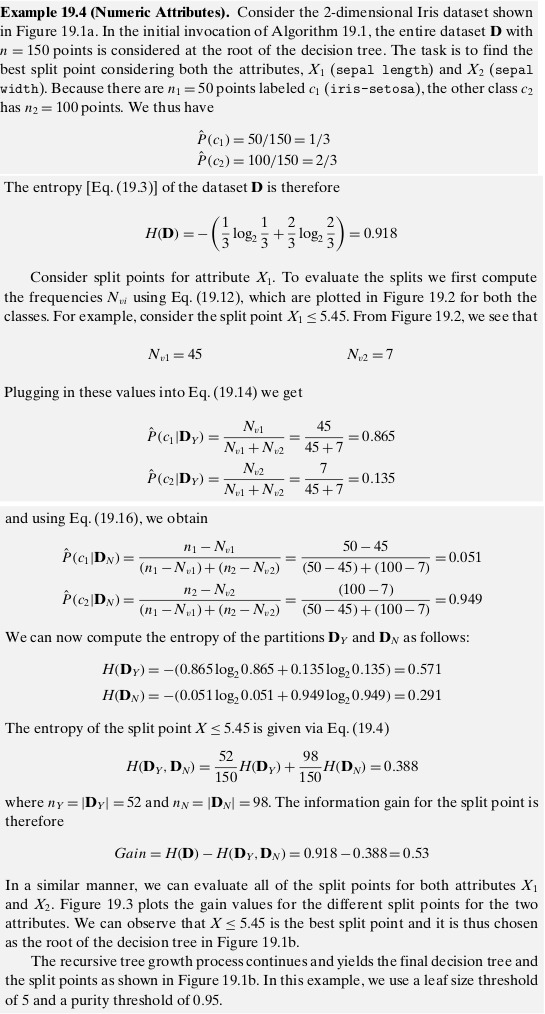
\includegraphics[width=\textwidth]{Figures/dt11}}
\caption{\label{fig:figure}Solution for Numeric Attributes}
\end{figure}
\begin{figure}[H]
\centerline{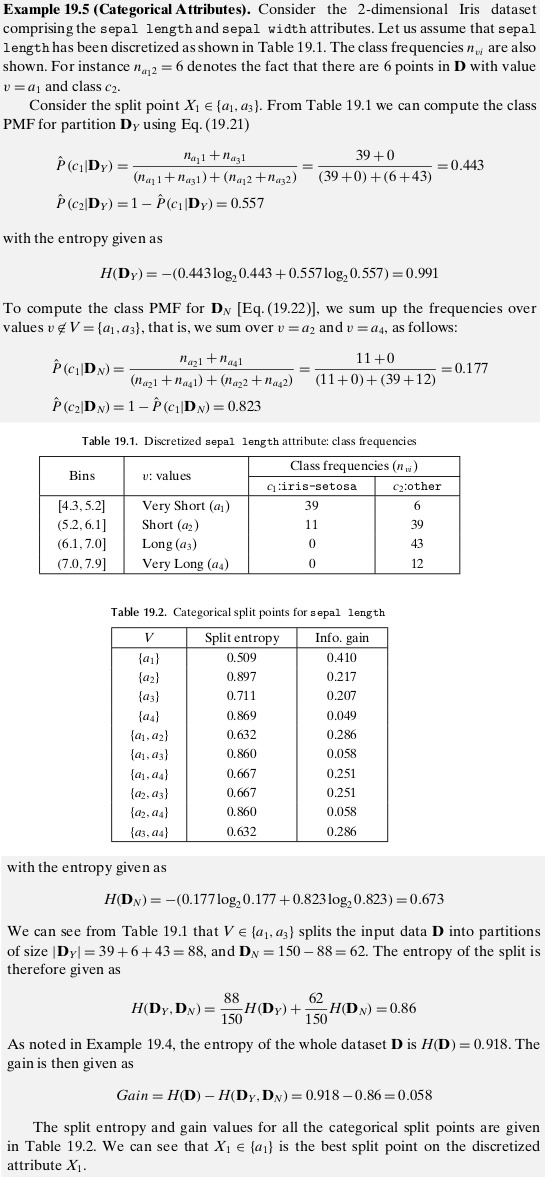
\includegraphics[width=0.9\textwidth]{Figures/dt12}}
\caption{\label{fig:figure}Solution for Categorical Attributes}
\end{figure}